\documentclass{beamer}

% Use the UiB theme
\usetheme{UiB}
% For strikethrough text using \sout
\usepackage[normalem]{ulem}

% For figures
\usepackage{graphicx}
\usepackage{tikz}
\usetikzlibrary{shapes.geometric,positioning,shapes.symbols,overlay-beamer-styles}

\usepackage{listings}
\usepackage{xcolor}
\usepackage{color}
\usepackage{generators/listings-golang}
\usepackage{generators/listings-haskell}
\usepackage{generators/listings-magnolia}
\usepackage{generators/listings-typescript}
\usepackage{amsmath}

% Presentation metadata
\title{Developing a zero-core modular IDE}
\subtitle{Creating a zero-cost IDE; you get what you pay for}
\author{Nils Michael Fitjar}
\institute{University of Bergen}
\date{\today}

\begin{document}
\section{Introduction}
\SectionPage

\begin{frame}
  \frametitle{Topic}
  \begin{itemize}
    \item About my thesis
    \item Modularity
    \item My implementation
    \begin{itemize}
      \item Modules
      \item Conclusion
      \item Demo
    \end{itemize}
  \end{itemize}
\end{frame}

\begin{frame}
  \frametitle{Thesis}
  \begin{itemize}
    \item For the technically inclined:
      \begin{itemize}
        \item Design and develop a \textit{zero-core}, \textit{modular}, \textit{IDE} 
      \end{itemize}
    \item For family members:
      \begin{itemize}
        \item Creating a tool for developers
      \end{itemize}
    \item Zero-core
      \begin{itemize}
        \item The tool gets all of its functionality from modules
      \end{itemize}
    \item Modular
      \begin{itemize}
        \item Functionality can be added by other developers (modules)
      \end{itemize}
  \end{itemize}
\end{frame}

\begin{frame}
  \frametitle{Integrated Development Environment (IDE)}
  \begin{itemize}
    \item All-in-one tool
    \item Single application with \textit{everything} a developer needs
      \begin{itemize}
        \item Manage files
        \item Compile and run code
        \item Run tests and show test reports
        \item Check for errors
        \item Warn about possible bugs
        \item Grammar check
      \end{itemize}
    \item Common features across languages and IDEs
    \item Might be unsuited for languages with unconventional features
    \item Can be solved with a module architecture
  \end{itemize}
\end{frame}

\section{Modularity}
\SectionPage

\begin{frame}
  \frametitle{Modularity in a programming language}
  \begin{itemize}
    \item Researches at UiB are experimenting with a programming language
    called Magnolia
    \item Created to experiment with novel language features inspired by
    academia
      \begin{itemize}
        \item For example: abstract algebra
      \end{itemize}
  \end{itemize}
\end{frame}

\begin{frame}
  \frametitle{Modularity in mathematics}
  \begin{itemize}
    \item Structure: A set, with an operation, and some \textit{rules} on the
    operation
    \item Magma is the \textit{simplest} structure in abstract algebra
    \item It is trivial to specify in Java using interfaces
    \item Semigroup, which is an exstension of magma, is more complicated
    \item With \textit{associativity} property (\textit{interface})
    \item More \textit{properties}, more interfaces
  \end{itemize}
\end{frame}

\begin{frame}
  \frametitle{Magma}
  \begin{figure}[H]
    \begin{subfigure}[h]{0.45\textwidth}
      \begin{equation}
        M = \{ a, b, c, \dots \}
      \end{equation}
      \begin{equation}
        a \odot b \in M
      \end{equation}
    \end{subfigure}
    \hfill
    \begin{subfigure}[h]{0.45\textwidth}
      \begin{center}
      \lstinputlisting
      [ language=Java
      ]{./code/magma.java}
  \end{center}
    \end{subfigure}
  \end{figure}
\end{frame}

\hidelogo

\begin{frame}
  \frametitle{Semigroup}
  \begin{figure}[H]
    \begin{subfigure}[h]{0.45\textwidth}
      Associativity (Semigroup)
      \begin{equation}
        (a \odot b) \odot c = a \odot (b \odot c)
      \end{equation}
    \end{subfigure}
    \hfill
    \begin{subfigure}[h]{0.45\textwidth}
      \begin{center}
        \lstinputlisting
        [ language=Java
        ]{./code/semigroup.java}
      \end{center}
    \end{subfigure}
  \end{figure}
  Addition with the natural numbers is a semigroup\footnote{Its technically a monoid, but a monoid is a semigroup with the identity property}
      \begin{center}
        $(1 + 2) + 3 = 1 + (2 + 3)$
      \end{center}
\end{frame}

\begin{frame}
  \frametitle{Magnolia: modularity in a programming language}
  \begin{itemize}
    \item Introduces something called \textit{concepts}
    \item Similar to a Java interface.
    \item A concept declares
      \begin{itemize}
        \item Types
        \item Operations on those types
        \item Axioms that specify the properties of the operations
      \end{itemize}
    \item Allows for reuse of logic, not just functions
    \item A concept can use other concepts, and rename the types and operations
      in the concept, this is called renaming
    \item Renaming is useful to vizualise for a Magnolia developer, but not a
    common feature in IDEs
  \end{itemize}
\end{frame}

\showlogo

\begin{frame}
  \frametitle{Magma example in Magnolia}
  \begin{figure}[H]
    \begin{subfigure}[h]{0.45\textwidth}
  \begin{center}
    \lstinputlisting
    [ language=Magnolia
    ]{./code/magma.mg}
  \end{center}
    \end{subfigure}
    \hfill
    \begin{subfigure}[h]{0.45\textwidth}
      \begin{center}
        $M = \{ a, b, c, \dots \}$
      \end{center}
      \begin{center}
        $a \odot b \in M$
      \end{center}
    \end{subfigure}
  \end{figure}
\end{frame}

\begin{frame}
  \frametitle{Semigroup example in Magnolia}
  \begin{figure}[H]
    \begin{subfigure}[h]{0.45\textwidth}
  \begin{center}
    \lstinputlisting
    [ language=Magnolia
    ]{./code/semigroup.mg}
  \end{center}
    \end{subfigure}
    \hfill
    \begin{subfigure}[h]{0.45\textwidth}
      Associativity (Semigroup)
      \begin{equation}
        (a \odot b) \odot c = a \odot (b \odot c)
      \end{equation}
    \end{subfigure}
  \end{figure}
\end{frame}

\begin{frame}
  \frametitle{Modularity in an IDE}
  \begin{itemize}
    \item IDEs functionality can be extended with modules
    \item Third party code to be executed/interpreted
      \begin{itemize}
        \item Tailor made Scripting Language
          \begin{itemize}
            \item Vim Script (Vim)
          \end{itemize}
        \item An already existing programming language
          \begin{itemize}
            \item Lua (NeoVim)
            \item JavaScript (VS Code)
            \item Java/Kotlin (Eclipse/IntelliJ)
          \end{itemize}
      \end{itemize}
  \end{itemize}
\end{frame}

\begin{frame}
  \frametitle{The current Magnolia IDE}
  \begin{itemize}
    \item Directly integrated with the Magnolia Compiler
    \item Made using an (now) old version of Eclipse
    \item Uses (now) deprecated Eclipse plugins
    \item Installation process is complex
    \item In INF220, two weeks is set aside for students to install it
    \item But has functionality to show renaming
  \end{itemize}
\end{frame}


\section{Planning}
\SectionPage

\begin{frame}
  \frametitle{Features}
  \begin{itemize}
    \item Easy to extend (with modules)
      \pause
      \begin{itemize}
        \item Low bar to create a module
        \pause
        \item Easy to reason about how modules work together
        \pause
      \end{itemize}
  \end{itemize}
\end{frame}

\begin{frame}
  \frametitle{Goals}
  % TODO: Should probably make these points more concrete
  \begin{itemize}
    \item Simple installation, for multiple OSes
      \pause
    \item Easy for the next \sout{sucker} developer to change core functionality
      \pause
      \begin{itemize}
        \item Good CI-CD
        \pause
        \item Good documentation
        \pause
      \end{itemize}
    \item Have a good module developer experience
      \begin{itemize}
          \pause
        \item Language Agnostic Module Architecture
          \pause
        \item Good debugging tools
      \end{itemize}
  \end{itemize}
\end{frame}

\begin{frame}
  \frametitle{What Is A Module?}
  \begin{itemize}
    \item Third Party Code to be executed/interpreted
      \pause
      \begin{itemize}
        \item Tailor made Scripting Language
          \pause
          \begin{itemize}
            \item Vim Script (Vim)
              \pause
          \end{itemize}
        \item An already existing programming language
        \pause
          \begin{itemize}
            \item Lua (NeoVim)
            \pause
            \item JavaScript (VS Code)
            \pause
            \item Java/Kotlin/Clojure (Eclipse/IntelliJ)
          \end{itemize}
      \end{itemize}
  \end{itemize}
\end{frame}


\section{Modeling a Module}
\SectionPage

\begin{frame}
  \frametitle{How To model A Module?}
  \begin{itemize}
    \item A module needs to:
      \pause
      \begin{itemize}
        \item Initialize some state
        \pause
        \item Update the state based on events
        \pause
        \item Change the view based on the state
      \end{itemize}
      \pause
    \item Module architecture is inspired by Elm and MVC
      \pause
    \item A module should be \textit{pure}
  \end{itemize}
\end{frame}

\hidelogo

\begin{frame}
  \frametitle{Scrapped Architectures}
  \begin{figure}
    \centering
    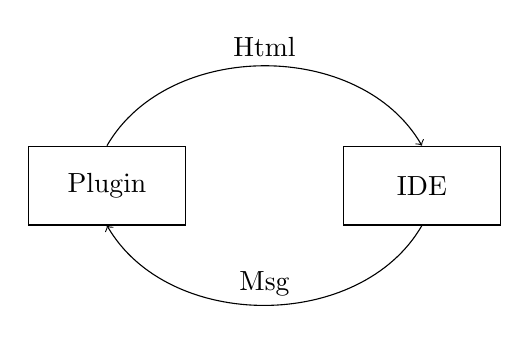
\begin{tikzpicture}
  % Nodes
  \node (p) [rectangle, draw, minimum height=1cm, minimum width=2cm] at (0, 0) {Plugin};
  \node (i) [rectangle, draw, minimum height=1cm, minimum width=2cm] at (4, 0) {IDE};
  % Arrow
  \draw[->] (p.north) to[out=60, in=120] node[midway, above] {Html} (i.north);
  \draw[->] (i.south) to[out=-120, in=-60] node[midway, above] {Msg} (p.south);
  % Header
\end{tikzpicture}


    \caption{Example Module Architecture}
    \label{fig:moduleArchitecture}
  \end{figure}
\end{frame}

\showlogo

\section{Implementation struggles}
\SectionPage

\begin{frame}
  \frametitle{Blasingly Fast Memory Leakage}
  \begin{itemize}
    \item The Rust ABI is not protected by their SemVer notation
      \pause
    \item This means that even a patch to the Rust compiler can break a
      Rust Module
      \pause
    \item Can be fixed by using a Rust Library: \textit{abi\_stable}
      \pause
    \item Had to use `ManuallyDrop` for more complex types, which disables
      the automatic drop
      \pause
    \item Fixed by having Rust modules only reference the state, meaning
      after update and view, the module can be safely dropped
  \end{itemize}
\end{frame}

\begin{frame}
  \frametitle{I Need Super Computer Time For My Featureless App}
  \begin{itemize}
      \pause
    \item JavaScript is more \textit{unsafe} than Rust, due of a lack of typing
      \pause
    \item Need to decode the output from the modules, and catch any exceptions
      \pause
    \item When implementing the init to update to view - cycle, I tested with
      a \textit{basic} module, which should only display "Hello, World!"
      \begin{itemize}
          \pause
        \item The module initialized the state
          \pause
        \item It rendered the view
          \pause
        \item Somehow triggered an update
          \pause
        \item Which triggered a re-render
          \pause
        \item Which triggered an update
          \pause
        \item Which triggered a re-render
          \pause
        \item \dots
      \end{itemize}
  \end{itemize}
\end{frame}

\hidelogo

\begin{frame}
  \frametitle{I Need Super Computer Time For My Featureless App}
  \begin{figure}
    \centering
    \includegraphics[width=0.9\textwidth]{./pics/memory-allocation-zoomed.png}
    \caption{140.6594 Terabytes of memory}
  \end{figure}
\end{frame}

\showlogo
\begin{frame}
  \frametitle{Module V.1 - Final.Final}
  \begin{itemize}
    \item Everything* is a module
      \pause
    \item Modules can \textit{invoke} modules
      \pause
    \begin{itemize}
      \item Init - Returns a set of modifications
    \end{itemize}
    \pause
    \item Pros
    \pause
    \begin{itemize}
      \item Modular
        \pause
      \item Modules can \textit{invoke} other modules
    \end{itemize}
    \pause
    \item Cons
    \begin{itemize}
        \pause
      \item Complex to implement
    \end{itemize}
  \end{itemize}
\end{frame}

\begin{frame}
  \frametitle{Module Type}
  \begin{center}
    \lstinputlisting
    [ language=Haskell
    ]{./code/module-example.hs}
  \end{center}
\end{frame}


\begin{frame}
  \frametitle{Event Type}
  \begin{center}
    \lstinputlisting
    [ language=Haskell
    ]{./code/module-example-event.hs}
  \end{center}
\end{frame}


\begin{frame}
  \frametitle{Counter Example}
  \begin{center}
    \lstinputlisting
    [ language=Haskell
    ]{./code/module-example-counter.hs}
  \end{center}
\end{frame}


\begin{frame}
  \frametitle{Event Handler}
  \begin{center}
    \lstinputlisting
    [ language=Haskell
    ]{./code/module-example-counter-handler.hs}
  \end{center}
\end{frame}


\input{./sections/03_conclusion}

\end{document}
